\chapter{Podstawy teoretyczne}
\section[Symulacja komputerowa][Symulacja komputerowa]{Symulacja Komputerowa}

\subsection{Wstęp}
\par{
Ludzkość od zarania dziejów stara się analizować otaczający ją świat. Nie bez powodu. Zrozumienie zasad wg. funkcjonuje otaczająca nas rzeczywistość zdaje się znacząco ułatwiać naszą egzystencję co w prostej linii prowadzi do tego, że samo dążenie do zgłębienia prawideł świata da się wytłumaczyć odwołując się bezpośrednio do ewolucji - osobniki lepiej rozumiejące otaczający świat potrafią lepiej się mierzyć z pojawiającymi się w nim przeciwnościami.
}

\par{
Zasadniczo ludzkie badania działają na dwóch płaszczyznach - dążą do przewidywania przyszłości i pozwalają podejmować coraz lepsze reakcje na bieżące zdarzenia.
}

\par{
Przez wiele lat ludzie prowadzili rozliczne badania starające się wyjaśniać naturę świata - z początku nieco chaotycznie (co nie znaczy, że bez znaczących sukcesów) - u zarania nauki w starożytnej Grecji, gdy cała nauka zamknięta była w jedną dziedzinę nazywaną ogólnym mianem Filozofii.
Wraz z rozwojem ludzkości nasze podejście do nauki jako takiej ewoluowało. I tak już w XVII wieku Kartezjusz wysuwał postulaty, że podstawą nauki powinny być pewne abstrakcyjne narzędzia jak matematyka i logika na bazie których buduje się teorię innych dziedzin. Współczenie niewiele odsuneliśmy się od myśli Kartezjusza - podstawą naszych badań zdaje się być matematyka, na którą nakładane są inne dziedziny jak fizyka i chemia, których wypadkową są nauki przyrodnicze.
}

\par{
Warto zwrócić uwagę, że nasza nauka układa się wsosób warstwowy - kolejne warstwy pozwalają nam odcinać się od reguł obowiązujących w małej skali i budować torie dla skali większej. Jest to szczególnie uzasadnione w świetle odkryć XX wieku, jak ogólna teoria względności.
}

\par{
Oczywiście nadal wiele naukowych tez ma charakter czysto empiryczny i często jest to wystarczające dla określonych zastosowań - w końcu po dziś dzień nauka służy ludziom a nie odwrotnie.
}

\par{
Mamy więc doczynienia z pozornym rozłamem nauki - z jednej strony formalizmy pozwalające na precyzyjny, spójny i co najważniejsze - jednoznaczny, opis określonych zjawisk. Z drugiej strony badania empiryczne, na podstawie których często wyszukuje się potencjalnych dróg rozwoju w sposób analityczny. Obie te metody uzupełniają się wzajemnie - niektórych badań praktycznych nie sposób zaplanować bez określonych reguł i znajomości niektórych torii a jednocześnnie niektóre teorie (w zasadzie większość) nie powstały by gdyby nie konkretne obserwacje rzeczywistości.
}

\par{
Symulacja komputerowa, zdaje się być odpowiedzią na drugą metodykę, która jednakowoż ściśle wykorzystuje specyficzny aparat matematyczny. Stosując ją wykorzystujemy bowiem teorie w pewnej skali, by odtworzyć zachowania i obserować ich skutki w innej (zwykle większej), np. symulując ruch cząsteczek cieczy wg. określonych fizyką zasad by obserwować zachowanie cieczy jako całości w określonych warunkach.
}

\par{
Czym jest więc symulacja komputerowa? Symulacja to proces, który pozwala przy użyciu reguł jednej skali obserwować zjawiska w innej. Słowo komputerowa odnosi się do konkretnej realizacji - z wykorzystaniem maszyn cyfrowych. Dobrym podsumowaniem ukazującym funkcję symulacji komputerowej zdaje się być poniższy schemat przedstawiający trzy filary współczesnej nauki wg. prof. Michała Kleibera.
\begin{center}
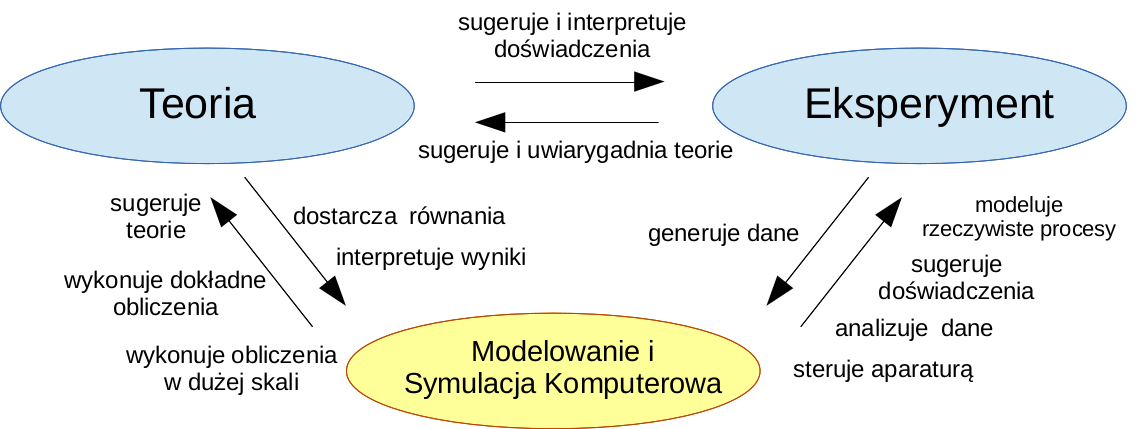
\includegraphics[width=\textwidth,keepaspectratio]{img/triada_poznania}
\textit{Trzy filary poznawcze współczesnej nauki [5].}
\end{center}
}

\subsection{Filozofia symulacji komputerowej}

\subsubsection{Postulat Laplace'a}
\par{
W roku 1814 Pierre Simon Laplace opublikował \textit{Essai philosophique sur les probabilites} (fran. \textit{Filozoficzny esej na temat prawdopodobieństwa}), w którym wysunął następujący postulat:
}
\par{
\textit{Umysł, który by znał siły działające w danej chwili w przyrodzie oraz wzajemne położenie wszystkich istotności, z których ona się składa, gdyby zdołał ująć je i poddać analizie - w jednym wzorze zawarłby ruchy największych ciał niebieskich i najdrobniejszych atomów. Nie byłoby dla niego nic niepewnego i zarówno przyszłość, jak i przeszłość świata byłyby obecne dla jego oka ...
}}
\par{
\textit{... Jesteśmy tak dalecy od chwili, kiedy poznamy wszystkie siły przyrody i różne formy ich oddziaływania, że nie byłoby godnym filozofa negowanie pewnych zjawisk jedynie dlatego, że nie można ich objaśnić przy obecnym stanie wiedzy. Jesteśmy zobowiązani do badania zjawisk tym dokładniej, im trudniej przychodzi nam uznać je za istniejące.}
}

\par{
Współczesna nauka odsunęła się nieco od tej koncepcji. Po pierwsze przyjmuje się (mając na względzie zasady fizyki kwantowej), że świat nie opiera sie o deterministyczne zasady - co w zasadzie obala postulat Laplace'a. Po drugie nastomiast, zgodnie z zasadą nieoznaczoności Heisenberga nie jest możliwe uzyskanie pełnego obrazu świata ponieważ każda jego obserwacja wpływa na jego stan - co uniemożliwia wykorzystanie postulatu Laplace'a w praktyce.
}
\par{
Obalenie teorii Laplace'a nie oznacza bynajmniej, że nie pozostaje ona poza światem nauki - nadal ma ona bardzo duże znaczenie filozoficzne oraz nadal aktualna pozostaje jej druga część. Ponadto, w wielu sytuacjach zakłada się, że zasada ta nadal obowiązuje - jednym z takich miejsc jest symulacja komputerowa.
}
\par{
Podstawą w zasadzie każdej symulacji komputerowej jest stan symulowanych obiektów oraz oddziaływania między nimi. Zakłada się, że symulator zna \textbf{wszystkie} zasady obowiązujące w symulowanym świecie jak i stan wszystkich obiektów w nim występujących i w związku z tym jest w stanie określić przyszłość symulowanego układu - jest to stan, o którym wspominał Laplace'a, a symulator można by w tym kontekście potraktować jako demona Laplace'a. Warto zwrócić uwagę, że w podejściu takim nie ma nic zdrożnego, ani sprzecznego ze współczesną nauką - przedewszystkim dlatego, że ograniczenie symulacji do ciągu przyczyn i skutków nie obniża zwykle jej wartości w kwestii celu jaki się przed nią stawia.
}

\subsubsection{Precyzja komputerów}
\par{
Kolejnym problem w pewien sposób uniemożliwający przyrównanie rzeczywstości do symulacji komputerowej jest fakt, że współczesne komputery przechowują dane w sposób skwantowany (binarny). W związku z tym nie sposób opisać na nim danych o charakterze ciągłym z dowolną precyzją.
}
\par{
Choć zdawać by się mogło, że w świetle współczesnych badań, ograniczenie to przestaje mieć sens, ponieważ przyjmuje się, że wszelkie zjawiska w przyrodzie mają charakter kwantowy, to należy wziąć pod uwagę jak małe są kwanty o których mówi ta teoria.
}
\par{
Długość Plancka (czyli minimalna obserwowalna we wrzechświecie odległość) wyniosi 
\begin{center}
$l_P = c \ t_P = \sqrt{\frac{\hbar G}{c^3}} = 1,616 199(97) \times 10^{-35} m$
\end{center}
co oznacza, że aby zapisać na komputerze dokładne położenie obiektu w trójwymiarowej kostce o boku długości jednego metra potrzebowali byśmy ok. $3.5 \times 10^{65}$ terabajta pamięci. Przy obecnej technologii zdaje się więc, że dokładność komputera jest zasadniczym problemem uniemożliwiającym dokładne odwzorowanie rzeczywistości.
}

\subsubsection{Praktyczne znaczenie ograniczeń}
\par{
W praktyce, wyżej wymienione ograniczenia nie są zwykle krytyczne. Zazwyczaj bowiem symulacja ma za zadanie upraszczać wygląd rzeczywistości, a więc nadmierna precyzja jest w wręcz niewskazana.
}
\par{
Warto jednak zdawać sobie sprawę, że symulacja komputerowa jest jedynie pewnym przybliżeniem rzeczywistości i z samej swojej natury obarczona jest zasadniczym błędem - i własnie \textbf{znalezienie takiego sposobu symulacji by błąd w możliwie małym stopniu wpływał na aspekty istotne z punktu widzenia celu symulacji zdaje się być istotą jej projektowania.}
}

\subsection{Zastosowanie symulacji}

\subsubsection{Przewidywanie zdarzeń}
\par{
Podstawowym zdaniem stawianym przed symulacjami komputerowymi zdaje się być przewidywanie różnego rodzaju zdarzeń. Znając zasady wg. których funkcjonują pewne zjawiska, jesteśmy w stanie do pewnego stopnia określić jak będą rozwijały się te zjawiska w przyszłości.
}
\par{
Niektóre z tych zjawisk potrafiliśmy przewidywać już przed erą symulacji komputerowej - albo przy użyciu klasycznego aparatu matematycznego albo przy użyciu własnej intuicji i doświadczenia. Jednak symulowanie zjawisk w celu przewidywania ich rozwoju przenosi przewidywanie przyszłości na zupełnie nowy poziom.
}
\par{
Na symulację możemy wpływać - tj. sprawdzać jak będzie reagowała na poszczególne bodźce ze świata zewnętrznego. Możemy także sterować jej przebiegiem - tj. w miejscach gdzie pojawia się niepewność związana z metodyką symulacji wybrać konkretny wariant rozwiązania problemu.
Dzięki temu, jesteśmy w stanie, w którkim czasie wytworzyć i przeanalizować wiele sceneriuszy wydarzeń i na podstawie tych doświadczeń podejmować działania (w szczególności realne działania prewencyjne).
}
\par{
Przykładem tego rodzaju zastosowań jest symulowanie przebiegu huraganu, pozwalające przewidywać jego rozwój, kierunek i szybkość przemieszczania się w zależności od licznych, często samych w sobie trudnych do przewidzenia okoliczności. Na podstawie tego rodzaju symulacji uruchamia się służby kryzysowe w odpowiednich rejonach, informuje się mieszkańców o zagrożeniu, czy zarządza ewakuację.
}

\subsubsection{Badania i eksperymenty}
\par{
Drugi typ zastosowań ma ścisły związek z badaniami naukowymi.
Opisując model pewnych zjawisk, przy użyciu symulatora jesteśmy w stanie sprawdzać reakcję całego układu na naszą ingerencję jak i obserwować jego zachowanie w stanie zamkniętym. Tego rodzaju badanie może często uzmysławiać pewne zjawiska w innej skali, niż ta na której rozpatrywany jest układ w modelu symulacji.
}
\par{
Przeprowadzanie niektórych eksperymentów w świecie realnym jest często problematyczne, kosztowne lub wręcz niemożliwe. Symulowanie eksperymentów zdaje się pozwalać w znacznym stopniu usprawniać badania a także wskazywać kierunki dalszego rozwoju. Jednocześnie najbardziej udane eksperymenty często powtarza się w rzeczywistości by uzyskać bardziej precyzyjny i pewny obraz.
}
\par{
Przykładem zastsowania w tym sektorze może być np. symulacja zbiornika z wodą na poziomie pojedyńczych cząsteczek by symulować jej zachowanie w konkretnych sytuacjach (np. uderzenie). Mając do dyspozycji taki symulator możemy zaobserować jak reaguje tafla wody na uderzenie i np. wysnuć teorię na temat związku długości fali na wodzie z siłą uderzenia.
}

\subsubsection{Testowanie}
\par{
Często spotykanym problemem, na który napotykają inżynierowie jest niemożność testowania ich rozwiązań w realnych warunkach. W takich sytuacjach z pomocą często przychodzą komputerowe symulacje. Dostarczają one danych do badań, lub pozwalają obserwować reakcje układu na działanie wdrażanego systemu.
}
\par{
Symulator opisywany w niniejszej pracy został stworzony z myślą o właśnie takim zastosowaniu. Ma on za zadanie generować dane wyjściowe dotyczące ruchu w środowisku miejskim przeznaczone jako wejście dla systemu śledzenia obiektów, który przystosowany został do pracy z realnymi danymi.
}
\par{
Rozwiązanie wykorzystujące symulator jest tańsze, szybsze oraz znacznie prostsze i może w znacznym stopniu wyprzedzać bieżące czasy.
Zebranie realnych danych na temat pojazdów poruszających się po mieście jest zadaniem nie łatwym. Kamery z funkcją rozponawania obiektów są dopiero raczkującą technologią a ich umieszczenie w całym mieście jest bardzo kosztowne. Umieszczenie ludzi spisujących odpowiednie, jest mało precyzyjne, i obarczone innym rodzajem błędów niż odczyty z kamer. Uzyskanie realnych danych potrzebnych do testowania skuteczności systemu śledzenia zdaje się więc być praktycznie niemożliwe.
}
\par{
Z pomocą przychodzą symulatory - za ich pomocą możemy wytworzyć takie dane, jakich powinna nam dostarczyć hipotetyczna kamera. Nałożyć na nie odpowiednie szumy. I zapisać razem z o wiele szerszymi danymi realnymi pozwalającymi analizować skuteczność wykorzystanych rozwiązań.
}
\par{
Dzięki temu, praca nad systemami śledzenia może postępować niezależnie od prac nad systemami monitoringu. Takie podejście sprawia że w sytuacji stworzenia i wdrożenia odpowiedniej realnej bazy sprzętowej będzie istniało już gotowe oprogramowanie mogące w pełni wykorzystać jej możliwości.
}
\par{
Wykorzystanie symulatorów do testowania zdaje się pozwalać na oszczędzanie dużej ilości zasobów i może prowadzić do skrócenia czasu badań pozwalając na unikanie kłopotliwych przygotowań do realnego testowania w trakcie koncepcyjnego opracowywania projektowanego systemu.
}

\subsubsection{Wizualizacja (także interaktywna)}
\par{
Ostatnim, acz nie najmniej istotnym z zastosowań symulatorów jest tworzenie wizualizacji w tym wizualizacji interaktywnych.
}
\par{
Organoleptyczne przekazywanie informacji jest bardzo istotne z punktu widzenia funkcjonowania człowieka - dane dostarczone w sposób nieprzetworzony są zwykle niezrozumiałe lub wymagają dużych nakładów czasu by wyciąganąć z nich potrzebne informację. Ponieważ często symulator ma za zadanie zaprezentować ogólny pogląd na symulowane zjawisko, typowo wraz z symulatorem dostarczany jest system pozwalający zwizualizować jego pracę.
}
\par{
Praktyczne zastosowanie tego rodzaju tandemu zdaje się być bardzo szerokie. Pozwala to na prezentowanie sedna złożonych zjawisk, ułatwia przekazywania informacji, pozwala na obserwowanie zjawisk, do których odruchowej analizy człowiek jest całe życie przyzwyczajany. Dzięki temu często w sposób heurystyczny jesteśmy w stanie wyznaczyć pewne prawidłowości, których zasadność często sprawdzana jest dokładnie albo analitycznie albo z wykorzystaniem tego samego symulatora i dołączonego do niego modułu analizującego dane.
}
\par{
Prezentując dane przy użyciu odpowiedniej wizualizacji, jesteśmy w stanie przekazać złożone informacje w sposób intuicyjnie zrozumiały. Jest to cenna właściwość szczególnie dla edukacji czy wszelkiego rodzaju ciał doradczych współpracujących z podmiotami nie operującymi naukową nomenklaturą.
}
\par{
Powołując się ponownie na przykład symulacji cząstek wody by obserować ich powierzchnię, wynikiem takiego symulatora było by zapewne położenie poszczególnych cząstek wody. Jednak chcąc widzieć realną powierzchnię - często z uzyskanych danych wytworzymy trójwymiarowy obraz dający nam wrażenie jakbyśmy pracowali z realną cieczą.
}
\par{
Wizualizowanie wszelkich zjawisk zdaje się być nierozłącznie związane z ich symulowaniem i stanowi istotny element a w wielu sytuacjach cel egzystencji symulatorów jako takich.
}

\subsection{Model symulacji komputerowej}
\subsubsection{Definicja modelu}
Modelem w symulacji komputerowej nazywamy zasady, wedle których funkcjonuje symulacja, uwzględniający wszelkie zmienne wejściowe i wyprowadzający z nich zmienne wyjściowe z uwzględnieniem upływu czasu.
\par{
W literaturze [3] można spotkać następującą, nieco bardziej ścisłą definicję:
Model \textit{to operator przekształcający zadane zmienne wejściowe X(t) w zmienne wyjściowe Y(t) czyli 
\begin{center}
$Y(t) = H_{t} \times X(t).$
\end{center}
}
}.

\subsubsection{Oczekiwane cechy modelu}
\par{
Przed modelami do symulacji najczęściej stawiane są trzy wymagania [2,4]:
\begin{itemize}
\item Wymaganie jednoznaczności - oznacza to, że operator modelu jest zależnością funkcyjną tzn. że jeden zbiór danych wejściowych daje dokładnie jedną odpowiedź.
\item Wymaganie spójności (rozwiązywalności) - oznacza to, że elementy modelu nie przeczą sobie nazajem (są matematycznie spójne).
\item Wymaganie stabilności - wymaganie to, oznacza, że niewielkie zmiany danych wejściowych nie powinny pociągać za sobą gwałtownych zmian w danych wyjściowych. Należy jednak zwrócić uwagę, iż niekiedy symulowany system posiada właściwości przeczące tej zasadzie - nietrudno wyobrazić sobie na przykład symulację nacisku na jakiś obiekt, który po przekroczeniu pewnej krytycznej wartości siły nacisku łamie się, powodując diametralną zmianę wyglądu całego systemu (w wyniku reakcji łancuchowej). 
\end{itemize}
}

\subsection{Taksonomia modeli}
\par{
Literatura [2,3,4] podaje wiele kryteriów podziału modeli, poniżej zestawiono najbardziej ostre spośród nich.
}

\subsubsection{Podział ze względu na istnienie czasu}
\par{
\begin{itemize}
\item model dynamiczny - znacznie bardziej popularny, upływ czasu jest uwzględniany w modelu i ma wpływ na wartości zmiennych wyjściowych.
\item model statyczny - nie uwzględnia upływu czasu lub wartosci zmiennych wyjściowych nie zależą od niego w żaden sposób.
\end{itemize}
}

\subsubsection{Podział ze względu na model czasu}
\par{
Dotyczy tylko modeli dynamicznych.
\begin{itemize}
\item model ciągły w czasie - istnieje możliwość wyznaczenia wartości parametrów wyjściowych dla dowolnej chwili czasowej.
\item model dyskretny w czasie - istnieje możliwość wyznaczenia wartości parametrów końcowych tylko dla przeliczalnego zbioru chwil czasowych.
\end{itemize}
}

\subsubsection{Podział ze względu na determinizm}
\par{
\begin{itemize}
\item model deterministyczny - dla danego stanu początkowego daje zawsze taki sam wynik.
\item model niedeterministyczny - wynik działania modelu nie jest zdetermininowany w momencie zadania stanu wejściowego.
\end{itemize}
}
\par{
Warto mieć na względzie, że modele niedeterministyczne niejako stoją w sprzeczności z postulatem Laplace'a jak i z postawionym wyżej wymaganiem jednoznaczności. Należy jednak pamiętać, że w typowym przypadku narzędziem programistycznym dla symulacji operującej na modelu niedeterministycznym będzie symulator liczb pseudolosowych, który choć wykazuje cechy probabilistyczne charakterystyczne dla liczb losowych, w rzeczywistości bazuje na deterministycznych zdarzeniach - w praktyce więc każda komputerowa implementacja symulatora będzie miała charakter deterministyczny.
}

\subsubsection{Podział ze względu na oddziaływanie ze światem zewnętrznym}
\par{
\begin{itemize}
\item model autonomiczny - tworzy zamknięty układ i nie uwzględnia żadnych możliwości interakcji z jego zewnętrzem.
\item model nieautonomiczny - pozwala na dostarczanie bodźców (pobudzeń, wartości) z zewnątrz, które mają wpływ na zmienne wyjściowe.
\end{itemize}
}

\subsubsection{Podział ze względu na rodzaj związków między wejściem a wyjściem}
\par{
\begin{itemize}
\item model liniowy - zmienne wyjściowe są związane ze zmiennymi wejściowymi przy użyciu liniowych funkcji.
\item model nieliniowy - wykorzystuje funkcje nieliniowe do obliczania wartości parametrów wyjściowych.
\end{itemize}
}

\subsubsection{Podział ze względu na sposób tworzenia}
\par{
\begin{itemize}
\item model dedukcyjny - reguły modelu pochodzą na podstawie teorii opisującej modelowane zjawisko.
\item model empiryczny - reguły są tworzone na podstawie obserwacji zachowań modelowanego zjawiska, tak by model miał podobne obserwowalne właściwości.
\end{itemize}
}

\subsection{Modelowanie}
\par{
Proces tworzenia modeli pewnych zjawisk (np. na potrzeby symulacji komputerowej) nazywany jest modelowaniem. Proces ten, stanowi często wyzwanie dla przystępujących do niego inżynierów ze względu na bardzo wysokość złożoność zagadnień jak i konieczność dobierania miejsc, które model będzie upraszczał względem rzeczywistości, tak by zachować zasadność tworzenia modelu.
}

\subsubsection{Aspekty tworzenie modeli}
\par{
Przystępując do modelowania jakichkolwiek zjawisk poprawnym podejściem jest zwrócenie uwagi na następujące aspekty [2]:
\begin{itemize}
\item \textbf{cel} - celowi tworzenia modelu powinny być podporządkowane wszystkie związane z nim działania. Należy pamiętać, że to model istnieje dla celu a nie odwrotnie. Cel symulacji stanowi punkt odniesienia, do którego należy często powracać i podporządkowywać mu decyzje podejmowane podczas modelowania.
\item \textbf{poziom uproszczenia} - model z samej swojej natury musi być pewnym uproszczonym odpowiednikiem wycinka rzeczywistości. Jego stopień skomplikowania nie może być zbyt wysoki, przez względ na dostępne metody praktycznej implementacji symulacji oń opertej. Z drugiej strony wybranie modelu nadmiernie uproszczonego moze prowadzić do zagubienia pewnych specyficznych zachowań symulowanego zjawiska - co może fałszować obraz symulacji. Dobrym określeniem porządanego stopnia uproszczenia modelu mogą być słowa Alberta Einsteina: \textit{Wszys­tko po­win­no być tak pros­te, jak to tyl­ko możli­we, ale nie pros­tsze.}
\item \textbf{potrzeby eksperymentu} - niezywkle często zdarza się, że zjawisko modelowane jest z zamiarem wykorzystania do ściśle określonego eksperymentu. Mając taką świadomość, jesteśmy w stanie łatwiej dobrać możliwe uproszczenia, a co ważniejsze pozbyć się wielu niepotrzebnych zależności z proponowanego modelu.
\item \textbf{poprawność} - model uznaje się za poprawny, jeśli poddany każdemu możliwemu wejściu zachowa się wystarczająco podobnie do realnego zjawiska poddanego bodźcom odpowiadającym temu wejściu. Określenie, czy dane wyjście jest wystarczająco podobne do wyjścia realnego jest decyzją jaką podejmuje modelujący mając na względnie różne aspekty modelu a w szczególności cel jego tworzenia. Zależności jakie powinny zachodzić w poprawnym modelu przedstawia poniższy rysunek.
\par{
\begin{center}
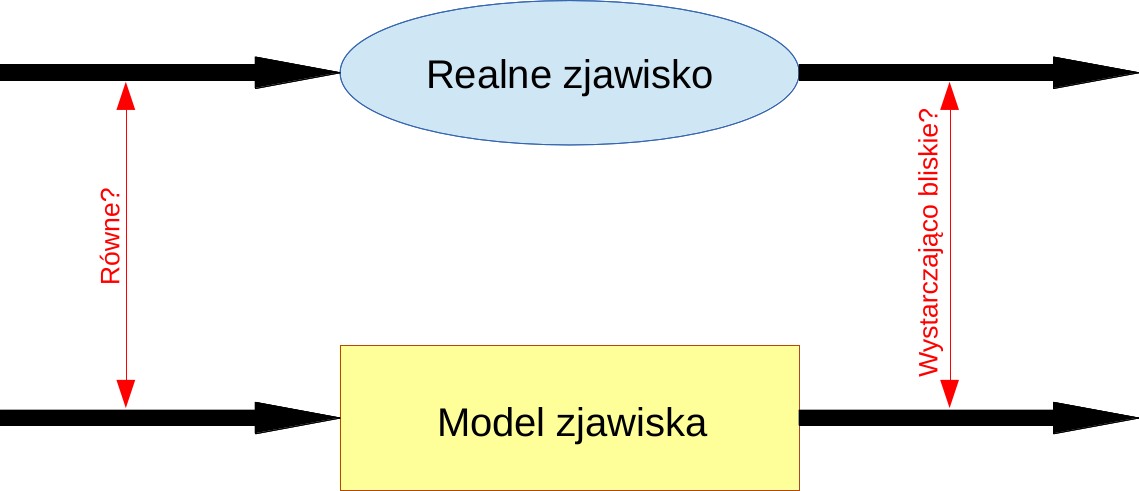
\includegraphics[width=\textwidth,keepaspectratio]{img/poprawnosc_modelu}
\textit{Popraność modelu względem modelowanego zjawiska [2].}
\end{center}
}
\item \textbf{przydatność} - model uznawany jest za przydatny gdy jego złożoność rośnie wolniej niż wykładniczo względem ilości zmiennych wykorzystywanych do jego opisu [2]. Modele zagadnień o złożoności wykładniczej mogą być poprawne, jednak ich precyzyjny opis jest często nieprzydatny i wymagane jest ich uproszczenie, by rozwiązywać symulowane zagadnienie z mniejszą dokładnością (np. heurystycznie) ale ciągle wystarczająco dobrze z punktu widzenia symulacji a jednocześnie w realnie dostępnym czasie.
\item \textbf{wiarygodność} - wiarygodność modelu określa na ile użytkownik jest przekonany o jego poprawności, szczególnie bazując na obserwacji wyników jego działania i organoleptycznym porównaniu tych wyników z realnym zjawiskiem. Wiarygodność modelu jest szczególnie istotna w przypadku symulacji przeznaczonych do wizualizacji określonych zjawisk.
\end{itemize}
}

\subsubsection{Zasadność modelu}
\par{
Model jako taki musi posiadać pewne cechy by był przydatny do jakichkolwiek zastosowań. Zastosowanie wyżej sformułowanych kryteriów doboru, powinno zapewnić, że model będzie właściwie sformułowany, jednak warto mieć dodatkowo na względzie dwa aspekty, wedle których można ocenić zasadność istnienia zaproponowanego przez nas modelu [4].
\begin{itemize}
\item Badanie modelu nie powinno być bardziej złożone od badanie właściwego zjawiska.
\item Model powinien (zwłaszcza w kwestiach związanych ze swoim celem) zachowywać się w sposób zbliżony do modelowanego zjawiska.
\end{itemize}
}


\section[Podstawy fizyczne][Podstawy fizyczne]{Podstawy fizyczne}

\subsection{Fizyczne modele dynamiki Newtona}
\par{
Do stworzenia odpowiedniego modelu symulacji komputerowej, oprócz znajomości metodyki modelowania wymagana jest znajomość teorii stojącej za modelowanym zjawiskiem oraz aparatu matematycznego dla niej odpowiedniego.
Ruch obiektów w środowisku miejskim jest związany ściśle z klasyczną dynamiką Newtona. W fizyce klasycznej funkcjonują dwa podstawowe modele uproszczone opisujące ruch obiektów wg. zasad dynamiki Newtona - model bryły sztywnej i punktu materialnego.
}

\subsubsection{Dynamika bryły sztywnej}
\par{
Model bryły sztywnej uwzględnia kształt i wymiary obiektu poruszającego sie w przestrzeni. Jego podstawą jest założenie, że każdy obiekt ma strukturę jednostajnej, sztywnej (niezmieniającej kształtu pod względem czynników zewnętrznych) oraz nie absorbującej energii bryły, która poddawana jest wszelakim oddziaływaniom.
}
\par{
W związku z tym, że model bryły sztywnej zakłada wymiarowość obiektów, posiadają one w tym modelu sześć stopni swobody, które określają ich położenie w trójwymiarowej przestrzeni:
\begin{itemize}
\item Trzy związane z ruchem postępowym
	\begin{itemize}
	\item szerokość (położenie na osi X)
	\item wysokość (położenie na osi Y)
	\item głębokość (położenie na osi Z)
	\end{itemize}
\item Trzy związane z ruchem obrotowym
	\begin{itemize}
	\item Kąt roll (obrót wokół osi X)
	\item Kąt yaw (obrót wokół osi Y)
	\item Kąt pitch (obrót wokół osi Z)
	\end{itemize}
\end{itemize}
}
\par{
\begin{center}
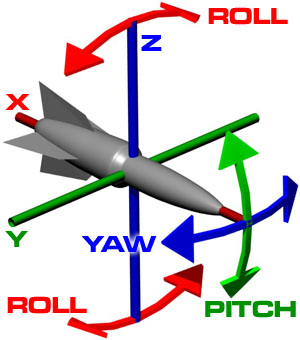
\includegraphics[]{img/xyz_ryp}
\end{center}
}
\par{
\begin{center}
\textit{Stopnie swobody bryły szytwnej, źródło: $http://www.projectrho.com/public\_html/rocket/controldeck.php$}
\end{center}
}
\subsubsection{Dynamika punktu materialnego}
\par{
Model punktu materialnego nie uwzględnia kształtu i fizycznego charakteru poruszającego się w przestrzeni ciała. W tym modelu przyjmuje się, że ciało (a więc cała masa) skupione jest w przestrzeni o zerowych wymiarach (punkcie). Tego rodzaju uproszczenie znacząco obniża skomplikowania rachunków związanych z ruchem ciał, jednak uniemożliwa rozpatrywanie ich ruchu obrotowego jak i nie jest w stanie bez dodatkowego wsparcia zapewnić spójnego opisu zderzeń obiektów (dwa punkty nie mogą się zderzyć gdyż nie mają wymiarów).
}

\par{
Ponieważ punkt materialny nie ma wymiarów, posiada zaledwie trzy stopnie swobody, związane z położeniem, nie jest natomiast opisywany przez obroty (jak bryła sztywna):
\begin{itemize}
\item szerokość (położenie na osi X)
\item wysokość (położenie na osi Y)
\item głębokość (położenie na osi Z)
\end{itemize}
}

\subsection{Rozwiązywanie równań dynamiki}
\par{
Posiadanie modelu fizycznego i odpowiedniej bazy matematycznej dla danego zjawiska pozwala na jego wykorzystanie, jednak wszelkie obliczenia związane z symulacją komputerową odbywać się będą przy użyciu maszyn cyfrowych. Koniecznym jest więc znalezienie sposobów numerycznego rozwiązywania problemów charakterystycznych dla wybranego modelu fizycznego - w tym wypadku dynamiki punktu materialnego.
}

\section[Systemy fuzji danych][Systemy fuzji danych]{Systemy fuzji danych}
\section[Modelowanie środowiska miejskiego][Modelowanie środowiska miejskiego]{Modelowanie środowiska miejskiego}
\subsection{Obiekty w środowisku miejskim}
\par{
Środowisko miejskie jest pojęciem bardzo kompleksowym i opisuje całokształt zjawisk związanych z funkcjonowaniem wszelkich obiektów fizycznych w granicach miast. Najważniejszymi elementami tego środowiska z punktu widzenia fuzji danych do celów śledzenia obiektów zdają się być jednak tylko te elementy, które bezpośrednio i znacząco wpływają na wyniki obserwacji.
}
\subsubsection{Obiekty statyczne}
\par{
Obiekty statyczne w środowisku miejskim to wszelkiego rodzaju elementy krajobrazu rozumiane jako bryły, a w szczególności zabudowania oraz roślinność. Obiekty te zdają się być stosunkowo proste do osadzenia w symulacji gdyż charakteryzują się niezmienną w czasie pozycją. Mają jednak one istotny i zmienny w czasie wpływ na obserwowane środowisko w związku z tym ich zaniedbanie może być przyjęte tylko po wcześniejszej analizie wpływu takiego uproszczenia modelu na cel symulacji.
}
\par{
Podstawowym pojęciem związanym z obiektami statycznymi jest przysłanianie. Warto zwrócić uwagę, że obiekty takie wpływają bezpośrednio na wynik obserwacji modelowanego środowiska w zależności od położenia obserwatora, czasu oraz pozycji innych obiektów. W związku z tym przy budowaniu modelu  obserwatorów środowiska należy uwzględniać jego interakcję z obiektami statycznymi.
}
\par{
Analogicznie sprawa wygląda jeśli chodzi o inne zaburzenia obserwacji spowodowane przez obiekty statyczne - odbicia, zacienienia itd. Tego rodzaju zjawiska również mogą być uwzględnione w modelu, jeśli ich występowanie wydaje się mieć istotny wpływ na wynik analizy problemu, do którego sporządzany jest model.
}
\par{
Innym aspketem związanym z symulowaniem elementów statyczych jest możliwość przewidzenia zderzeń pomiędzy obiektami dynamicznymi a statycznymi. W takiej sytuacji także obiekty statyczne muszą posiadać pewną fizyczną reprezentację by być w stanie wyznaczyć przebieg zdarzenia.
}
\subsubsection{Ścieżki}
\par{
Ścieżki są w zasadzie obiektami statycznymi, jednak o bardzo charakterystycznych właściowościach. Wyznaczają one bowiem potencjalne trasy po jakich poruszają się obiekty dynamiczne.
}
\par{
Reprezentacja fizyczna ścieżek zdaje się być relatywnie bez znaczeni. Warto jednak mieć na względzie, że w niektórych sytuacjach ich wygląd czy kształt może wpływać na efektywność obserwacji, np. czarny samochód może być trudniejszy do automatycznego wykrycia przez systemy rozpoznawania obrazu na czarnym asfalcie niż na jasnych betonowych płytach. Innym elementem związaną z fizyczną reprezentacją ścieżek może być np. śliskość, która wpływa na poruszające się po niej obiekty dynamiczne.
}
\par{
Modelując środowisko miejskie należy podjąć świadomą decyzję na temat reprezentacji fizycznej ścieżek - w wypadku celu tej pracy ich fizyczna reprezentacja w modelu zdaje się nie być istotna ponieważ praca ta nie służy analizie skuteczności pozyskiwania informacji. Nie wydaje się również żeby ich fizyczna reprezentacja miała znaczenie z punktu widzenia jakichkolwiek aspektów symulowanej przestrzeni. Warto zwrócić uwagę, że jeśli w przyszłości zajdzie potrzeba modelowania właściwości scieżek jako takich, można wykorzystać do tego celu typowy model obiektów statycznych, który zapewnia wszystkie właściwości potrzebne danej symulacji - jako że \textbf{ścieżka jest właśnie obiektym statycznym powiększonym o pewne dodatkowe właściwości}.
}
\par{
Podstawową właściwością ścieżki jest posiadanie początku i końca umieszczonego w przestrzeni. Dodatkowo ścieżkę charakteryzować mogą inne właściwości jak np.:
\begin{itemize}
\item Kierunek
\item Szerokość
\item Rodzaj obiektów, dla których jest przeznaczona
\end{itemize}
}
Te właściwości bezpośrednio wpływają na sposób poruszania się obiektów dynamicznych. Założeniem prezentowanego modelu jest bowiem, 
\subsubsection{}
\begin{itemize}
\item \textbf{Pojazdy} - 
\item \textbf{Piesi} - 
\end{itemize}



\subsection{Specyfika obserwacji}
\subsection{Szumy i niedokładności}
